\section{Adminsicht}

\subsection{Installation}
Das ausführbare jar an die gewünschte Stelle kopieren und zum Ausführen doppelt klicken.


\subsection{Start}
	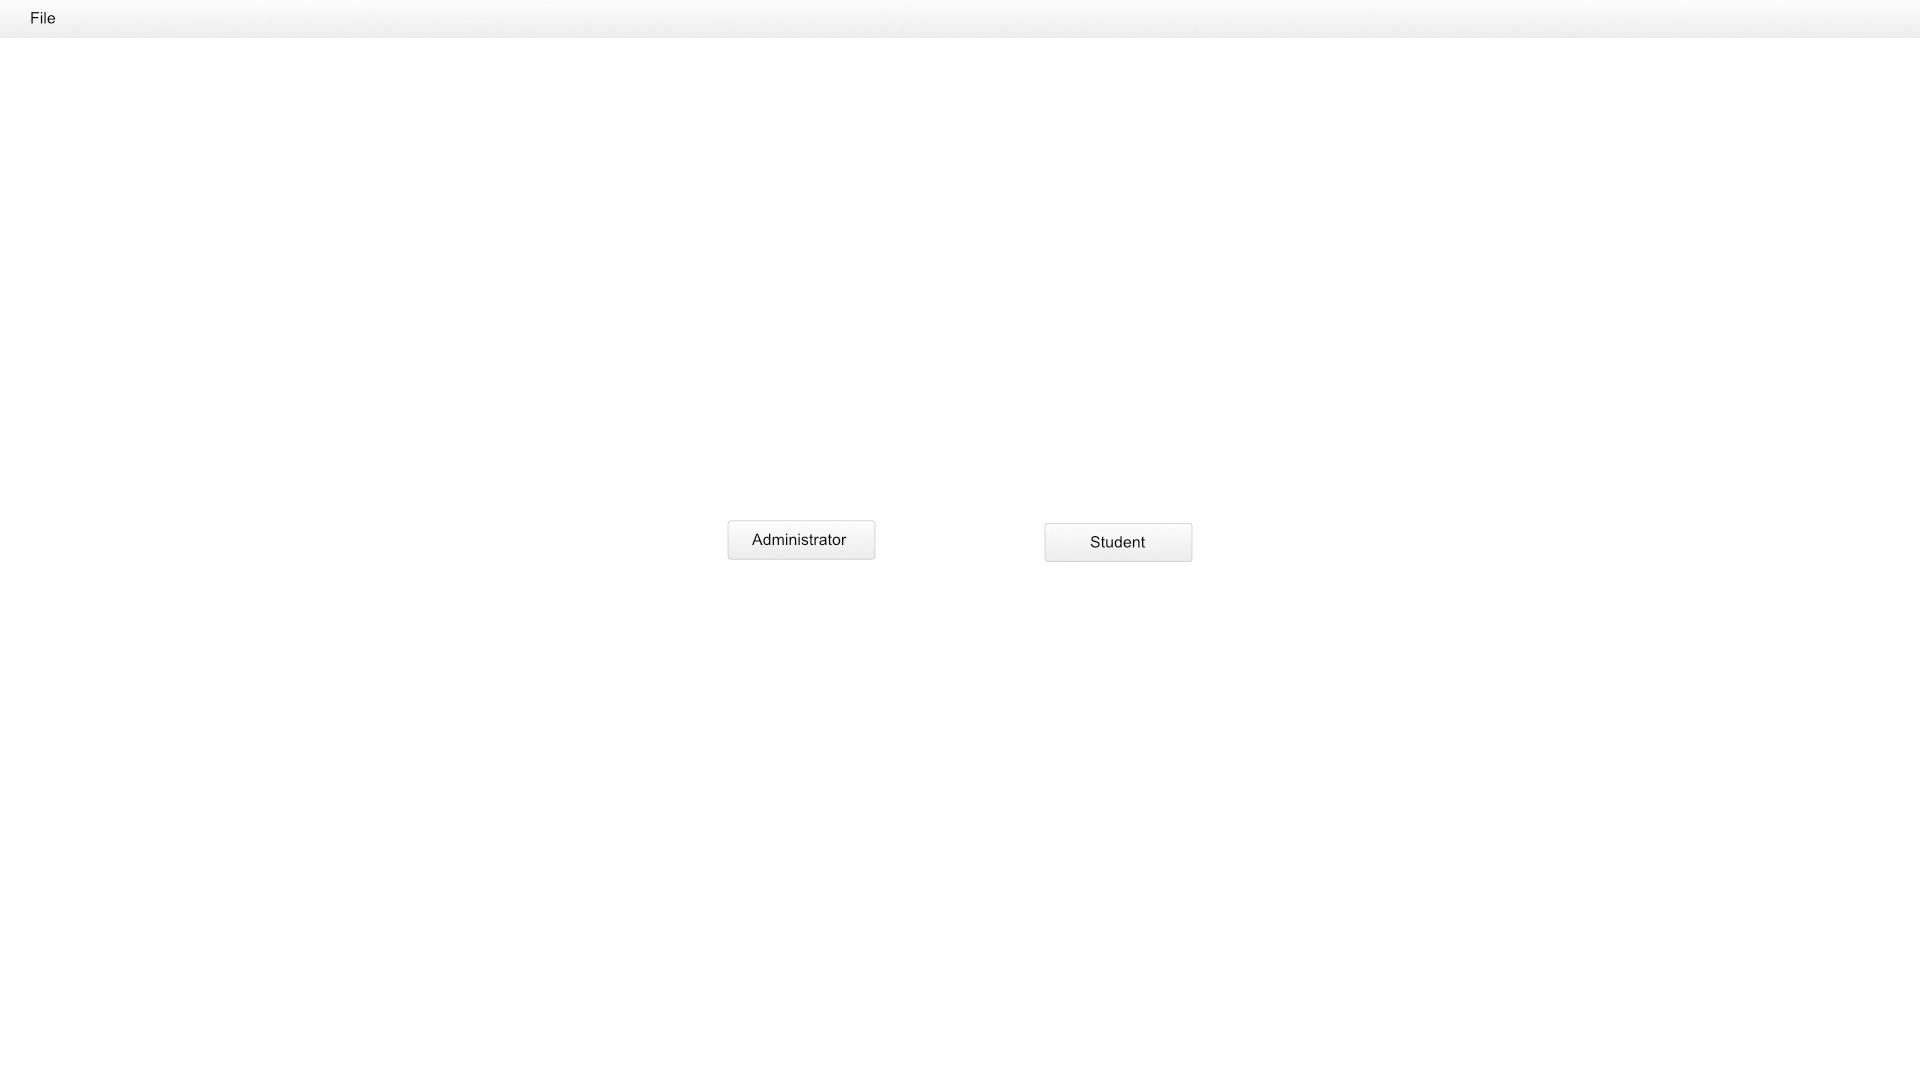
\includegraphics[width=\textwidth]{Bilder/Role-selection}
	\\
	\\
Dies ist das Startfenster der Anwendung. In diesem kann der Benutzer mit einem klick auf einen der angezeigten Buttons den Zugang auswählen welchen er nutzen möchte. Für die Benutzung der Anwendung als Administrator den Button \textit{Administrator} auswählen. 



\subsubsection{Einrichten}
	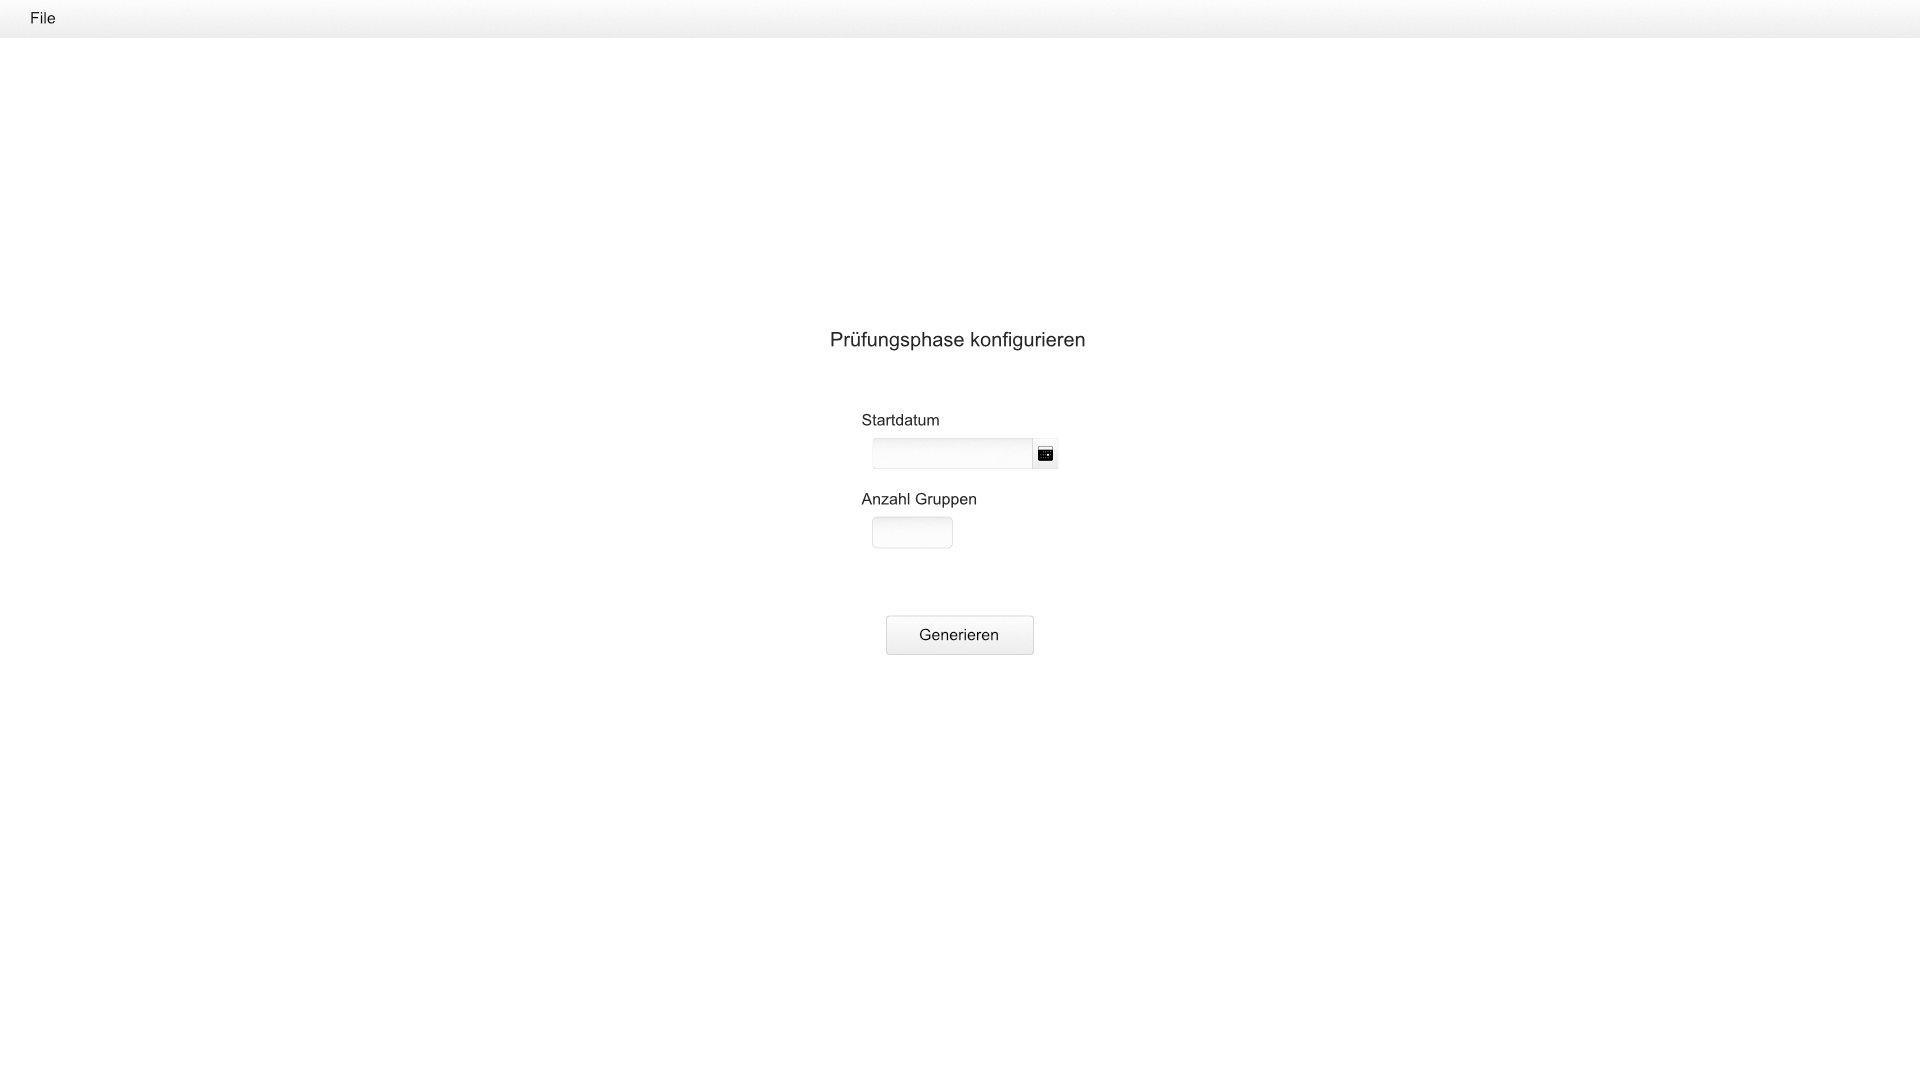
\includegraphics[width=\textwidth]{Bilder/Admin/Setup}
	\\
	\\
Um die Anwendung einzurichten klickt man den Punkt \textit{File} daraufhin öffnet sich ein Menü und wählt dort den Eintrag \textit{Termine und Gruppen generieren}. Damit öffnet sich ein neues Fenster. \\In das Textfeld \textit{Startdatum} wird der Beginn der Prüfungsphase eingetragen, wahlweise kann das Datum auch über das Kalender Icon neben dem Textfeld ausgewählt werden. In das Textfeld \textit{Anzahl der Gruppen} wird die Anzahl der Gruppen eingetragen die in der vorher festgelegten Prüfungsphase eine Präsentation halten. 
\\
\begin{wrapfigure}{R}{0.2\textwidth}
	\centering
	
\includegraphics[width=0.20\textwidth]{Bilder/Buttons/Generieren}
\end{wrapfigure}

Durch betätigen des Buttons \textit{Generieren} erstellt die Anwendung eine Listenübersicht für drei Wochen mit dem eingetragenen Datum als Startdatum.


\subsection{Gruppen}
	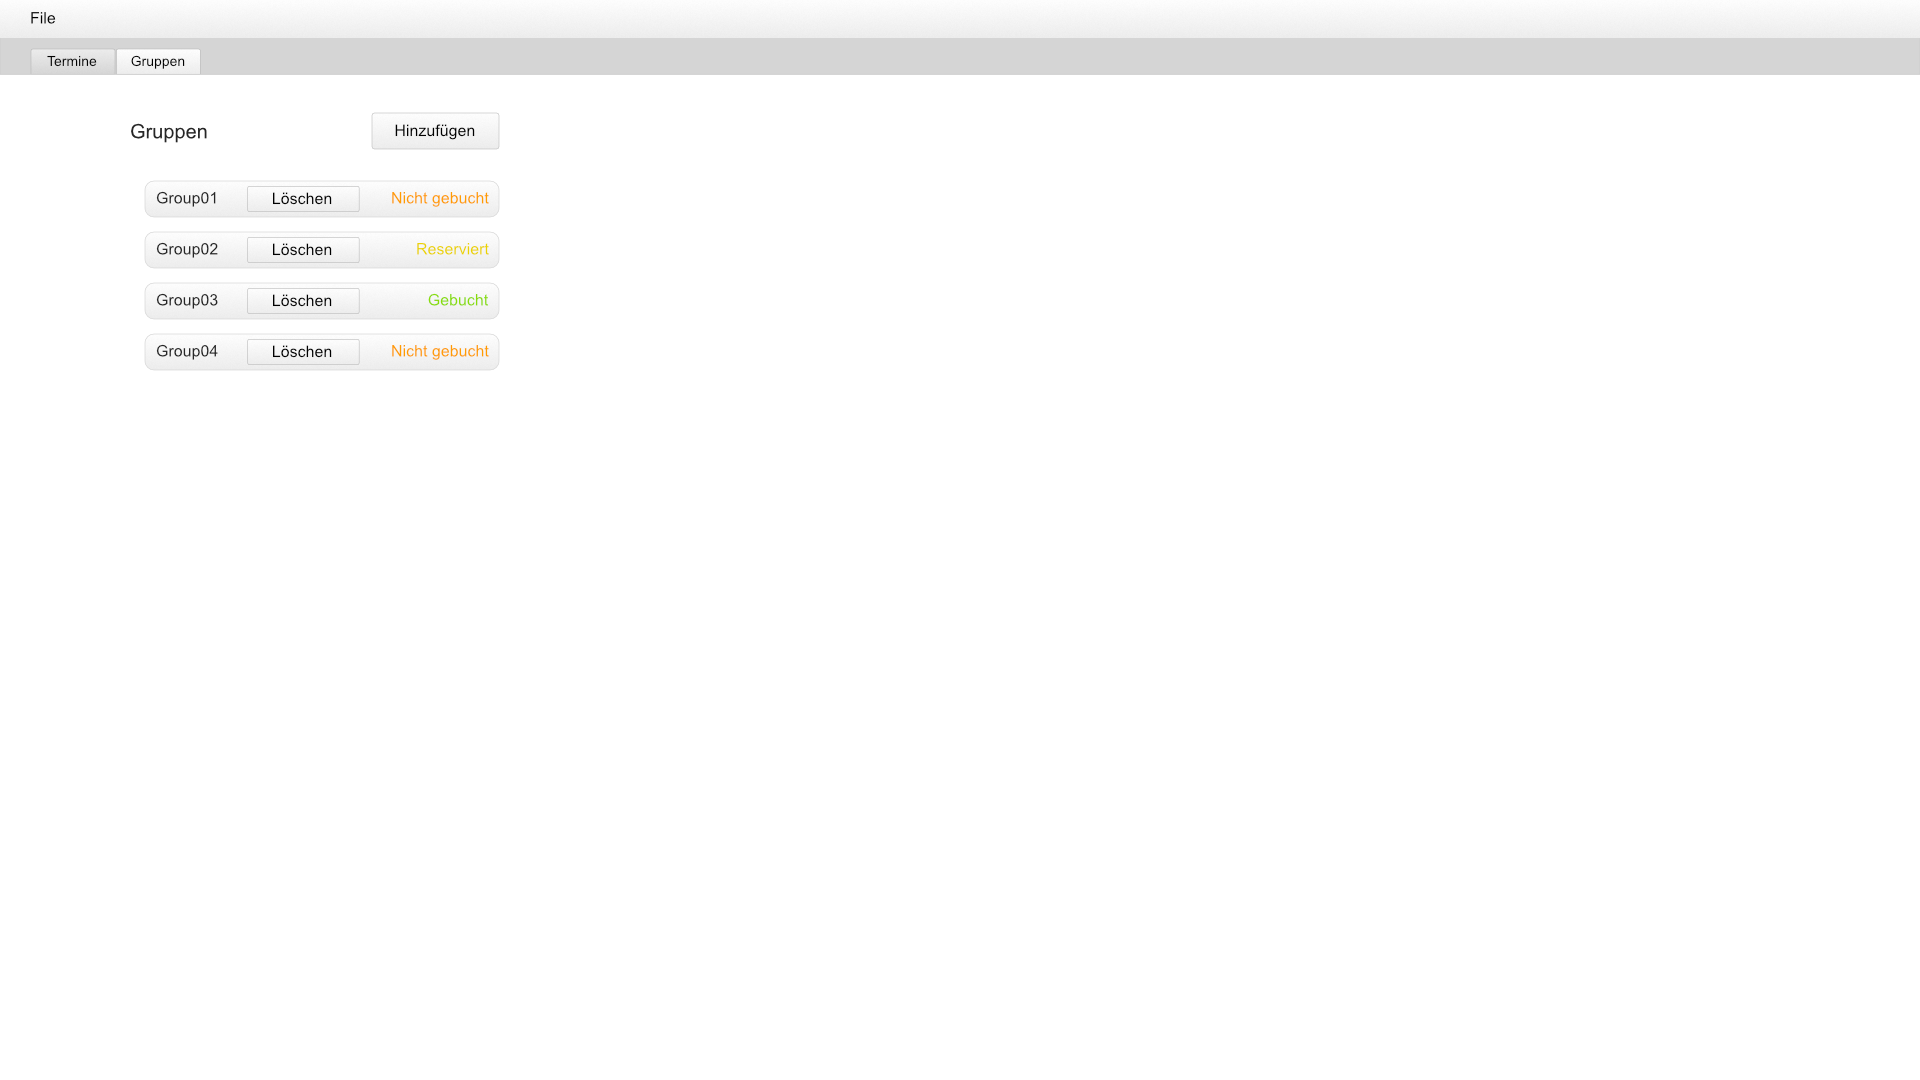
\includegraphics[width=\textwidth]{Bilder/Admin/Group-management}
	\\
	\\	
Im Tab Gruppen kann der Administrator mit dem Button \textit{Hinzufügen} eine neue Gruppe anlegen. Diese bekommt automatisch den Namen Gruppe mit einer fortlaufenden Nummerierung.\\Mit dem Button \textit{Löschen} können bereits vorhandene Gruppen gelöscht werden, Buchungen und Reservierungen der Gruppe löscht die Anwendungen automatisch.

\subsection{Termine}
	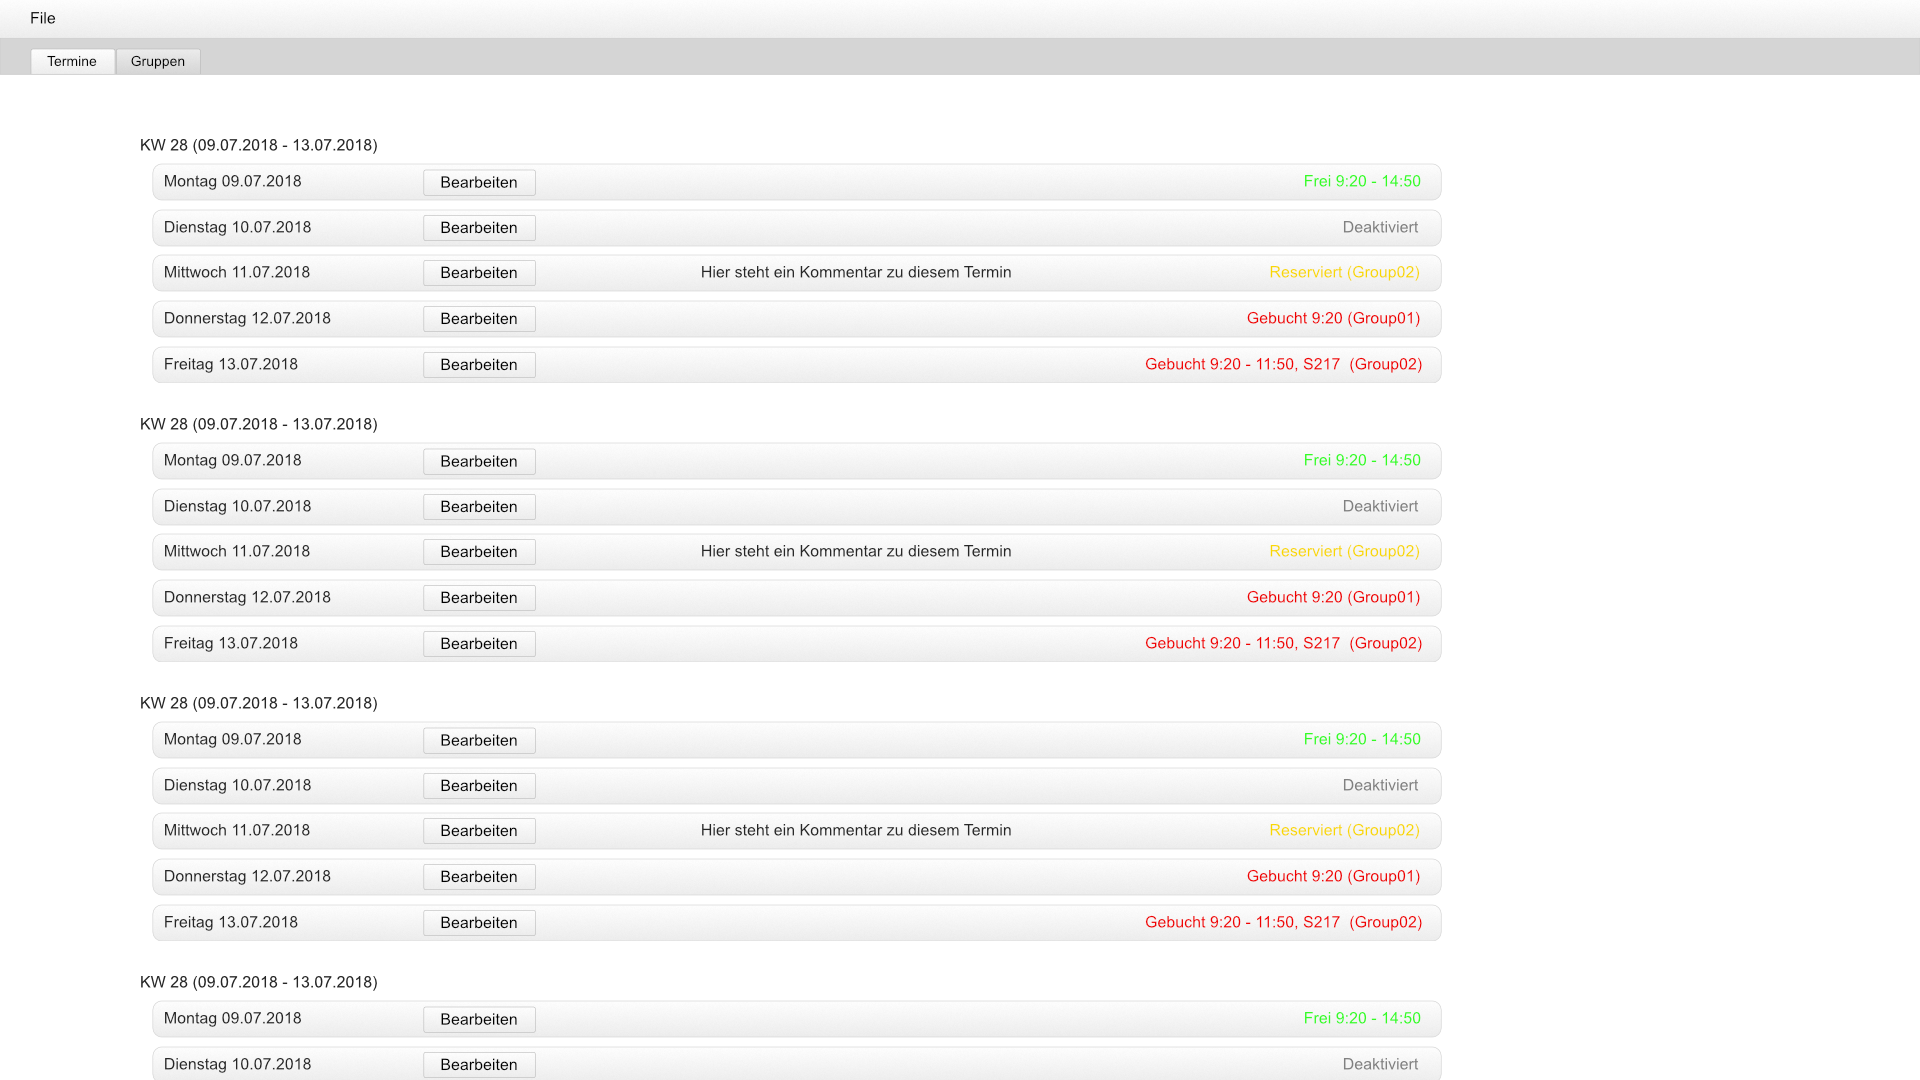
\includegraphics[width=\textwidth]{Bilder/Admin/Date-management-Admin}
	\\
	\\
In dem Tab Termine kann der Administrator die Listenübersicht der Wochen einsehen. Hier sind auch die Zustände der Tage eingetragen, sprich ob ein Tag
\begin{itemize}
	\item Frei 
	\item Deaktiviert 
	\item Reserviert 
	\item Gebucht
\end{itemize}
ist.
\\ Mit dem Button \textit{Bearbeiten} können die Tage bearbeitet werden. Es öffnet sich je nach Zustand ein entsprechendes Fenster.


\paragraph{Frei}
\begin{wrapfigure}{R}{0.2\textwidth}
	\centering
	\includegraphics[width=0.4\textwidth]{Bilder/Buttons_clicked/Admin_Edit-Button-no-Booking}
\end{wrapfigure}
Ist der Tag frei sprich es sind keine Buchen oder Reservierungen vorhanden öffnet sich ein Fenster. In diesem kann der Administrator die Zeiträume festlegen in welchen eine Buchung möglich ist, zusätzlich kann der Tag mit einer Bemerkung versehen werden. Eine Reservierung belegt den kompletten Tag daher wird in diesem Fall kein Zeitraum benötigt. 
\\Mit dem Button \textit{Deaktivieren} kann der Tag deaktiviert werden. Dies ist immer möglich auch wenn eine Reservierung oder eine Buchung vorhanden ist. Buchungen und Reservierungen löscht die Anwendung beim Deaktivieren automatisch.


\paragraph{Deaktiviert}
Ist ein Tag deaktiviert kann dieser mit klicken des Buttons \textit{Bearbeiten} und daraufhin mit betätigen des Buttons \textit{Aktivieren} wieder aktiv geschaltet werden.
In dieser Ansicht können außerdem wieder Bemerkung und Zeitfenster bearbeitet werden.
\\

\paragraph{Reserviert}
\begin{wrapfigure}{R}{0.2\textwidth}
	\centering
	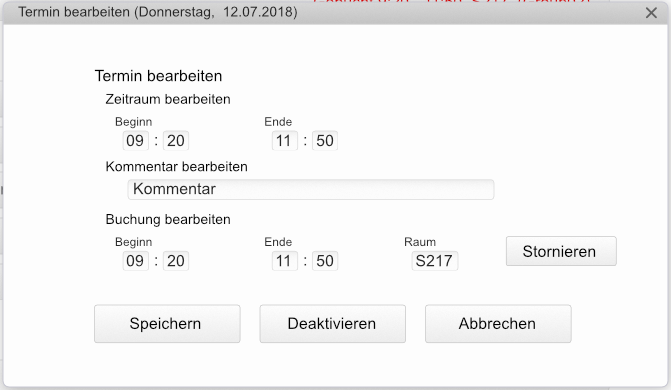
\includegraphics[width=0.4\textwidth]{Bilder/Buttons_clicked/Admin_Edit-Button-Booking}
\end{wrapfigure}
Wenn eine Reservierung vorhanden ist kann der Tag wie oben beschrieben bearbeitet werden. Zusätzlich kann der Administrator über den Button \textit{Stornieren} die Reservierung entfernen.

\paragraph{Gebucht}
Ist eine Buchung vorhanden kann diese wie oben beschrieben  storniert werden. Des Weiteren kann unter dem Abschnitt \textit{Buchung bearbeiten} eine konkrete Zeit und der Raum für die Präsentation eingetragen werden.  

\subsubsection{Speichern}
Mit klicken des Buttons \textit{Speichern} werden alle eintrage und Änderungen gespeichert und übernommen 
